\chapter{Overall System Design}
In this chapter we present the overall design of Media-Online Management(MOM). First we will present how we intend the users to use MOM. Then general concepts will be introduced which is an essential part of the system and will be mentioned several times hereafter. Thirdly the requirements of MOM will be explained in more detail. Finally the system architecture will be presented.    


\section{Media-Online Management} %name our system: temp name: Media-Online Management or MOM
The Media-Online Management (MOM) is the system that is our solution on the problem statement. To give an overview of the complete system a rich picture \citep{OOAD} have been made, see the figure \ref{fig:systemoverview}. The figure shows a home environment with a TV (media), computer and an internet connection, and it shows a server. 

There are two main use patterns. The first is a parent who manage their MOM using the website from the PC to add, change or delete system settings. This is pictured in the bottom left-side corner in figure \ref{fig:systemoverview}. 

The second use pattern is pictured in the upper left corner of the figure. It is a child user who wants to use a media which in this case is the television. But to watch television it need power and its power source is blocked by the controller. So the child needs to scan his tag and then the controller sends a message to the server which then reply whether the television can be turned on or not. When the child is done he must scan again such that points can be withdrawn from his user profile. If the child does not have any points he cannot turn on the television nor can he turn it on if a rule or permission does not allow it. If a parent wants to watch television without being restricted in any way he can make a rule that gives him unlimited access, but he would still need to scan his tag before and after using the television. \fixme{Vil vi lave en lille evaluering om vi synes det er fair at forældrene også skal scanne?}

\begin{figure}
	\centering
		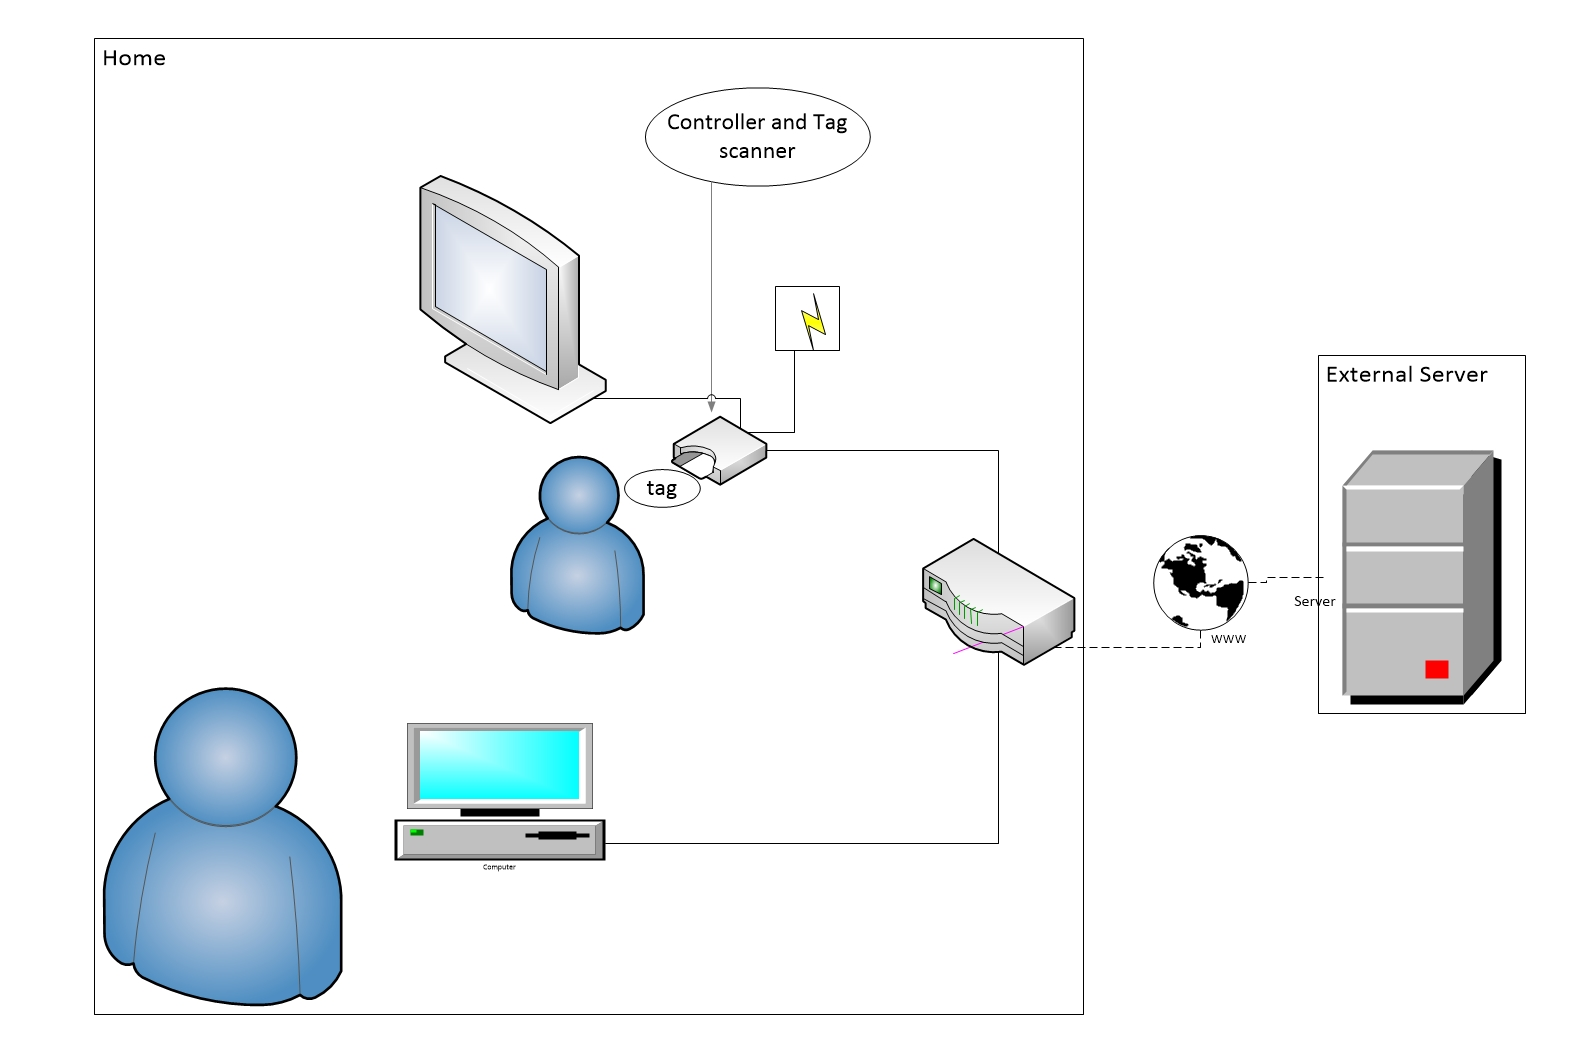
\includegraphics[width=1.00\textwidth]{images/systemoverview.jpg}
	\caption{system overview}
	\label{fig:systemoverview}
\end{figure}

On the server there will be a database, files that generate the website, a web service, and a daemon. These elements of the system will be explained further in section \vref{sec:RequirMOM} and after that the system architecture can be presented in section \vref{sec:sysArchitecture}. However, we need to explain some of the concepts that will be used in connection with this system.

\section{General Design Concepts}
%Go into detail about rules, permission, chores
In the Media-Online Management there are a few concepts that will be used through out the report. These are chore, permission and rules. The meaning of each will be explain in following sections.\fixme{Evt. refferance til intro afsnit, alt efter hvor meget det minder om hinanden. Men uanset er det godt med en opsang.}

\subsection{Chore}
A chore in MOM is a representation of a house chore that is to be done regularly. We have included chore into this system to encourage children to help with the house chores which gives more time for media as a reward. Therefore each chore needs a number of points which will be given when the child has done the house chore. 
An example on a house chore could be to take out the garbage, then the chore in MOM would have a name: 'take out garbage', possible a bigger description of the chore: 'remember to sort the garbage into the correct trash cans' and when the chore is done some points is given: '10'.  

One disadvantage about the chore design is that the parent needs to use the website to award the child with points for doing a chore. We would have liked to automate it further, but to limit the scope of the project this would be future work.  

\subsection{Permission}
Permissions in this system is a time period in which the child user is allowed to use a specific media. Permission is included in MOM to give parents an easy way of controlling which time periods during the day the media can be used by the child. This can help the parents to get the children to bed in time since they cannot use the medias unless the parent allows it. It would especially be useful if the child has medias in his room such that the parents do not need to check whether the media is turned off or not. 

The permission consist of:
\begin{itemize}
	\item a name of the permission
	\item a representation for the time period, which would need a from time and a to time. 
	\item a representation of days where the permission applies, which can be all days of the week or just some of them.
	\item a representation of when it should be repeated, which can be:
		\begin{itemize}
		\item weekly
		\item every second week
		\item every third week
		\item first in a month
		\item last in a month
		\end{itemize}
\end{itemize}

An example of a permission is Peter is allowed to use the TV each weekday in the time period 17:00 to 19:00. The permission in the system would then have a time 17:00 (FromTime), a time 19:00 (ToTime), the day representation 'Monday, Tuesday, Wednesday, Thursday, Friday', and it's repeated weekly.\fixme{Måske lidt for meget Database representation med Monday, Tuesdag...}


\subsection{Rule}
In the system a rule can be many things the following is just a few examples of rules:

\begin{itemize}
	\item any permission can also be written as a rule
	\item The first Monday in a month increase Peter's points by 100
	\item Mom and Dad's profiles have unlimited time and unrestricted access to any media
\end{itemize}

The rule has been included because it gives the parent users more powerful methods to control the use of medias in MOM. %and to control the profiles in the 
But there is one disadvantage with rules, it might be complicated for the user to understand how to use them. 
This means we must take care to design the concept of rules, so that it is easy to use and understand their effects.
%and how to construct a rule so the design of how the user can make a rule need to be though through carefully.

A rule should be connected to one or more user profiles since the rules otherwise would be unnecessary if no one should follow them. A rule consist of a name, a set of conditions and a set of actions. The conditions and actions will be explained further in the following sections.
	
\subsubsection{Condition}
A condition is used to decide when a rule is relevant which is when all conditions fits. A condition has a predefine name and when the user make a condition he will choose it from a list. The names is listed below together with the additional information that is required. 

\begin{description}
	\item[Timeperiode] when this is chosen the user can define a time period. It needs the same information as a permission, a from time, a to time, representation of days where the rule applies, and a representation of when it should be repeated. The time period can be either repeatable or nonrepeatable where the from time and to time is the only data required.
	\item[Timestamp] the condition has a timestamp as an additional information and an action should happen immediately after this timestamp have been reached. 
	\item[Controller on] this should check whether a given controller for a media is active. This needs to be connected to a controller.
	\item[Controller off] this should check whether a given controller for a media is not active. This needs to be connected to a controller.
	\item[True] This is always true.
\end{description}

Later in this chapter there will be some examples of rules which uses conditions.

\subsubsection{Action}
\label{subsubsection:action}
An action is something that can or should be done if all of the rule's conditions hold. An action always has a name, but as with the condition this name is not user defined. The user have a choice from a list which can be found in the description below with an explanation of what it does and what other information is needed for the action and which conditions it can be combined with.   

\begin{description}
	\item[Block user] it will block the profiles of all profiles connected to the rule. This action can be combined with Timestamp.
	\item[Activate user] it will activate or re-activate the profiles of all profiles connected to the rule. This action can be combined with Timestamp.
	\item[Add points] it will add points to all profiles connected to the rule. Here the number of points is needed. This action can be combined with Timestamp, Timeperiod(Repeateble).
	\item[Remove points]    This action can be combined with Timestamp, Timeperiod(Repeateble).
	\item[Set maximum of point] it will set a maximum for the number of points that a profile can have. Here a number representing the maximum points is also needed. This action can be combined with True.
	\item[Unlimited time] it will give the profile unlimited time to be spend on any media. This action can be combined with True and Timeperiod both repeatable and nonrepeatable.
	\item[Access any controller] it will give the profile access to any media in the system. This action can be combined with True and Timeperiod both repeatable and nonrepeatable.
	\item[Cannot access any controller] it will not give the profile access to any media. This action can be combined with True and Timeperiod both repeatable and nonrepeatable.
	\item[Access controller] it will give the profile access to a specific media. Here a controller need to be connected to the action. This action can be combined with any of the condition names.
	\item[Cannot access controller] it will block the user from using a specific media. Here a controller need to be connected to the action. This action can be combined with any of the condition names.
\end{description}
		
Since some of the action like 'Add points' should be done automatically without further contact with the user. A background process typically called daemon, is also needed in MOM but this will be explained further in section \ref{subsec:daemon}. 


\subsection{Permission and Rules Precedence}
It should be possible to override permissions and rules with another rule, but we need to establish priority among the permission and rules. 
For the overriding of the two to be relevant they need to overlap in time which mean that the condition should use Timeperiod or True. Also if it is a rule then it should have an action with the name 'Cannot access controller', 'Access controller', 'Cannot access any controller' or 'Access any controller' to be relevant. 

We came to the conclusion that rules always have precedence over permissions. But if it is two rules it is a more complex set of precedence rules. First to determine the precedence we look at the action's name. See figure \ref{fig:precendence} where the precedence graph is shown. Notice that the precedence for 'Cannot access controller' and 'Access controller' can be either way depending on the condition. 
  
\begin{figure}
	\centering
		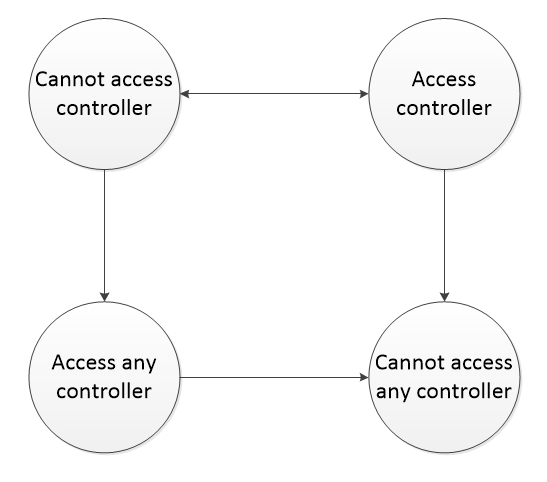
\includegraphics[width=0.75\textwidth]{images/precendence.jpg}
	\caption{Precedence of rules}
	\label{fig:precendence}
\end{figure}

When the condition determines the precedence we have different combinations:

\begin{itemize}
	\item If one is True and the other is Timeperiod then the rule with the Timeperiod has the higher precedence
	\item If both is True then Access controller has the precedence.
	\item If both is Timeperiod:
		\begin{itemize}
			\item If both is repeatable or non-repeatable then Access controller has the precedence
			\item If one is repeatable and the other is nonrepeatable then the rule with the nonrepeatable Timeperiod has the higher precedence.
		\end{itemize}
\end{itemize}

These precedence rules do not avoid all possible conflict but it limits them.  
	
\subsubsection{Examples of Rules}
In this section some examples of rules for a profile will be given.

The first example could be that the profile Peter gets point for each football training and the football training is Monday and Thursday from 18:00 to 19:30 each week. Then the action could be add 25 points to Peter when condition holds. The condition is from 19:30 to 19:30 where the day is 'Monday, Thursday' and it is repeated weekly. \\

The second example could be that Susan is grounded from the 2. December. In the system there will be a condition with Timestamp which is 2. December 2013 18:00
and an action that is 'Block user' such that she cannot use any media or gain points in this period. \\

If the parents should make a rule which give themselves unlimited time and access to any media. The condition would be True and the actions would be 'Unlimited time' and 'Access any controller'.\\\\

This conclude the general concepts that will be used through out the remainder of the report. Next further details about the requirements of MOM is described.  


\section{Requirements of MOM}
\label{sec:RequirMOM}

In the analysis we came to the conclusion that the following items is necessary for MOM: 
\begin{itemize}
	\item A device to toggle the power of an electronic media
	\item An individual key for each child that can be read by the device
	\item A website to set up rules, permissions and view/modify allowed usage of electronic media
\end{itemize} 


The first item is called controller in this system, the second is the tag and the last is the website on the computer. But also new components of the system is necessary. As explained in the previous section a daemon is needed to check the relevant rules and perform the appropriate actions if the conditions holds. Also during the following sections we find that a web service is needed. 

In the following sections the specification of the website, controller and tag, web service and daemon will be explained, before the design and implementation will be presented for each of them in the following chapters.  

\subsection{MOM's Website}
\label{subsection:momswebsite}
A Media-Online Management (MOM) owner needs a way to manage the system and for this a website will be made. There are several requirements for this website:

\begin{itemize}
	\item Register a new MOM together with a user profile which is a manager of this system
	\item Make it possible to add, edit and delete user profiles in an existing MOM 
	\item Make it possible to add, edit and delete Controllers from an existing MOM
	\item There should be a way to add, edit and delete Tags to the system. Also a tag should be connected to a user profile
	\item There need to be an option to add, edit and delete rules, permissions and chores from a system
	\item The user should be able to connect rules and permission with one or more user profiles. The connection should also be able to be removed without removing the rule or permission
	\item When a chore is done in the real world by a child profile then by connecting this profile to a chore, points should be added to his profile
\end{itemize}

There are also some requirements that is nice for the parents to use, but they are not essential for MOM system:

\begin{itemize}
	\item present the media consumption data as graphs or logs such that the parents easy can get an overview of their children's media consumption 
	\item present data from MOM in a calendar that shows rule and permission with profiles for whom this is relevant. The calendar should also show when a chore have been done and by who.
\end{itemize}

In chapter \fixme{insert ref} the design and implementation of the website will be presented in more detail. 
 

\subsection{Tag and Controller}
The tag used in this system is using Radio-frequency Identification (RFID). The tag need to be uniquely identified in MOM and it must uniquely identify its user. The tag is used in combination with the controller.

The controller is an Arduino which is connected to a tag reader. Like the tag it need to be uniquely identified in MOM. The controller must be able to do the following.

\begin{itemize}
	\item Read the data from the tag
	\item Send and receive messages from the server
	\item Control the power source of the media 
	\item Temporarily store the tag id that activated this controller
	\item Keep track of the time spent between activation of the media to its end
\end{itemize}
 
The design and implementation of the controller will be explained further in chapter \fixme{insert chapter ref}. 

The controller must communicate with the server and this is done via a web service.

\subsection{The web service}

The web service is used to parse the relevant data to the controller. Its requirements are:

\begin{itemize}
	\item Receive and send messages to the controller
	\item From a tag and controller it should be able to determine whether a user may use the media which is connected to the controller
	\item It must be able to subtract points from a user after he has been using a media
	\item It should able to calculate when a controller should be turned off because of a rule, permission or point.
\end{itemize}

The web service's design and implementation is explained further in chapter \fixme{ref to chapter}.


\subsection{Daemon}
The daemon is used to update data in the database from a rule which the user have made at some point. The daemon does not have any direct contact to a client. The daemon should handle any rule that is time determined so the condition is either Timestamp or Timeperiod. Then the daemon should do the appropriate action which could be add points to user or block a user.

The design and implementation of the daemon is presented in detail in chapter \fixme{ref to chapter}. 
 
\section{System Architecture}
\label{sec:sysArchitecture}
Now that all subsystem of the Media-Online Management have been presented the overall system architecture can be explained. MOM is using the client server architecture which is shown in the figure \ref{fig:serveroverview} \citep{OOAD}. This system has two types of client the first is a controller and the second is a computer where the user manages the system via the web site. The controller is depended on the web service on the server and the computer is depended on the web site. On the server there is the web site, web service and daemon which all are depended on the functions component, MySQLHelper class and data component. In the function component there are several functions to work on the data in the database and this component is depended on MySQLHelper because it should establish the database connection and parse the quires on to the database. 

\begin{figure}
	\centering
		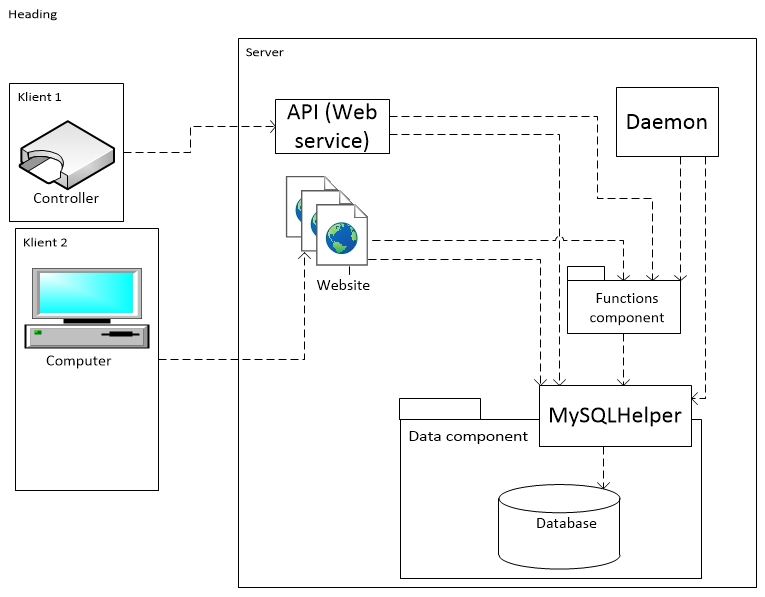
\includegraphics[width=1.00\textwidth]{images/serveroverview.jpg}
	\caption{system architecture}
	\label{fig:serveroverview}
\end{figure}

In the following chapters design and implementation of the web site, web service, deamon and database will be presented.

 


